\documentclass[serif,mathserif]{beamer}
\usepackage{etex}
\usepackage{amsmath, amsfonts, epsfig, xspace}
\usepackage{algorithm,algorithmic}
\usepackage{pstricks,pst-node}
\usepackage{multimedia}
\usepackage[normal,tight,center]{subfigure}
\usepackage{beamerthemesplit}
\usepackage{color}
\usepackage{mdframed}

\setlength{\subfigcapskip}{-.5em}
\usetheme{lankton-keynote}

\usepackage{graphicx,color}
% remove caption of figure
\usepackage[labelformat=empty]{caption}

\usepackage[none]{hyphenat} % hyphenation is ugly in slides
\usepackage{parskip}

\usepackage{relsize} % \smaller to change size

\usepackage{tikz}
\usetikzlibrary{calc}

\usetikzlibrary{arrows}

\newcommand{\TikzDraw}[2][]{
  \begin{tikzpicture}[overlay, remember picture, shift={(current page.center)}, #1]
    #2
  \end{tikzpicture}
}

\newcommand{\gridlines}{
  \TikzDraw{
    \draw[help lines,xstep=.2,ystep=.2,red!20] (current page.south west) grid (current page.north east);
    \draw[help lines,xstep=1,ystep=1,red] (current page.south west) grid (current page.north east);
    \foreach \x in {-15,-14,...,15} {
      \node [anchor=north, red] at (\x,0) {\tiny \x};
      \node [anchor=east,red] at (0,\x) {\tiny \x};
    }
  }
}

\newcommand{\DrawOnImg}[3][]
{
  \begin{tikzpicture}
    \node[anchor=south west,inner sep=0] (image) at (0,0){
      #2
    };
    \begin{scope}[x={(image.south east)},y={(image.north west)}]
      \ifthenelse{\equal{#1}{grid}}
                 {\draw[color=blue, style=dashed] (0,0) grid[xstep=.1, ystep=.1] (1.0001,1.0001);}
                 {}
                 #3
    \end{scope}
  \end{tikzpicture}
}


\author[Jiong Chen]{Jiong Chen}

\title[\hspace{2em}\insertframenumber/\inserttotalframenumber]{\huge A Chebyshev Semi-Iterative Approach for Accelerating Projective and Position-based Dynamics}

\date{December 9, 2015} %leave out for today's date to be insterted

% \institute{Zhejiang University}

\newcommand{\BOLD}[1]{\mathbf{#1}}
\newcommand{\BOLDG}[1]{\boldsymbol{#1}}
\newcommand{\PDIF}[2]{\frac{\partial #1}{\partial #2}}
\newcommand{\TODO}[1]{\textcolor{red}{#1}}
\newcommand{\TODOB}[1]{\textcolor{blue}{#1}}
\newcommand{\argmin}{\operatornamewithlimits{arg\min}}
\DeclareMathOperator{\tr}{tr}
\DeclareMathOperator{\cond}{cond}
\DeclareMathOperator{\ST}{s.t.}
\DeclareMathOperator{\diag}{diag}

\newmdtheoremenv{theo}{Theorem}

\definecolor{DARK}{RGB}{45, 33, 73}
\definecolor{LIGHT}{RGB}{119, 52, 106}
\definecolor{TEXTLIGHT}{RGB}{213, 207, 229}
\definecolor{TEXTDARK}{RGB}{66, 66, 66}
\definecolor{BULLET}{RGB}{179, 17, 102}
\definecolor{EM}{RGB}{179,17,102}

\begin{document}

\maketitle

\begin{frame}
 \frametitle{Background}
 \begin{itemize}
  \item Projective dynamics \TODO{\textit{[Bouaziz et al. 2014]}}
  \begin{equation*}
    \BOLD{x}_{t+1}=\argmin_{\BOLD{x}} \frac{1}{2h^2}\|\sqrt\BOLD{M}(\BOLD{x}-\BOLD{s}_t)\|^2+\sum_c\frac{w_c}{2}\|\BOLD{A}_c\BOLD{x}-\BOLD{\hat A}_c\BOLD{q}_c\|^2+\delta_c(\BOLD{q}_c)
  \end{equation*}
  \item Position-based dynamics \TODO{\textit{[M\"uller et al. 2007]}}
    \begin{itemize}
     \item[-] Eliminate $\frac{1}{2h^2}\|\sqrt\BOLD{M}(\BOLD{x}-\BOLD{s}_t)\|^2$
     \item[-] $\BOLD{A}_c = \BOLD{\hat A}_c = \sqrt \BOLD{M}$
     \item[-] Use Gauss-Seidel to solve the global step
    \end{itemize}
 \end{itemize}
\end{frame}

\begin{frame}
 \frametitle{Two Specific Examples}
 \begin{itemize}
  \item Fast mass spring system \TODO{\textit{[Liu et al. 2014]}}
  \begin{equation*}
   \begin{split}
    E(\BOLD{x})=T(\BOLD{x}; \BOLD{x}_t, &\BOLD{v}_t, \BOLD{M}, h)+ \sum_{(i, j)}\frac{w_{i, j}}{2}\|\BOLD{x}_i-\BOLD{x}_j-\BOLD{d}_{i,j}\|^2 \\
    &\ST \quad \|\BOLD{d}_{i,j}\| = r
   \end{split}
  \end{equation*}
  \item Geometric elastic model \TODO{\textit{[Chao et al. 2010]}}
  \begin{equation*}
   \begin{split}
    E(\BOLD{x})=T(\BOLD{x}; &\BOLD{x}_t, \BOLD{v}_t, \BOLD{M}, h)+ \sum_{t}\frac{w_t}{2}\|\BOLD{F}_t-\BOLD{R}_t\|_F^2 \\
    &\ST \quad \BOLD{R}_t \in SO(3)
   \end{split}
  \end{equation*}
 \end{itemize}
\end{frame}

\begin{frame}
 \frametitle{Solvers for Global Step}
 \TikzDraw {
  \node at (-1.75, 0) {\parbox[t]{0.75\textwidth}{
    \begin{itemize}
      \item Direct
      \begin{itemize}
      \item[-] Relatively expensive 
      \item[-] Cannot be accelerated by GPU.
      \end{itemize}
      \item Jacobi
      \begin{itemize}
       \item [-] Highly compatible with GPU.
      \end{itemize}
      \item Gauss-Seidel
    \end{itemize}
  }};
 }
\end{frame}

\begin{frame}
 \frametitle{PD and Jacobi method}
\end{frame}

\begin{frame}
  \frametitle{Chebyshev Approach}
\end{frame}

\begin{frame}
 \frametitle{Reproduced Results Summary}
  Direct+Chebyshev \& One Jacobi+Chebyshev
  \begin{itemize}
    \item \TODO{The estimation of $\rho$ has significant impact on the convergence.}
    \item $\rho_{tet}(0.87375) < \rho_{spring}(0.9992)$
    \TikzDraw {
      \visible<2> {
	\node at (-2.5, -1.3) {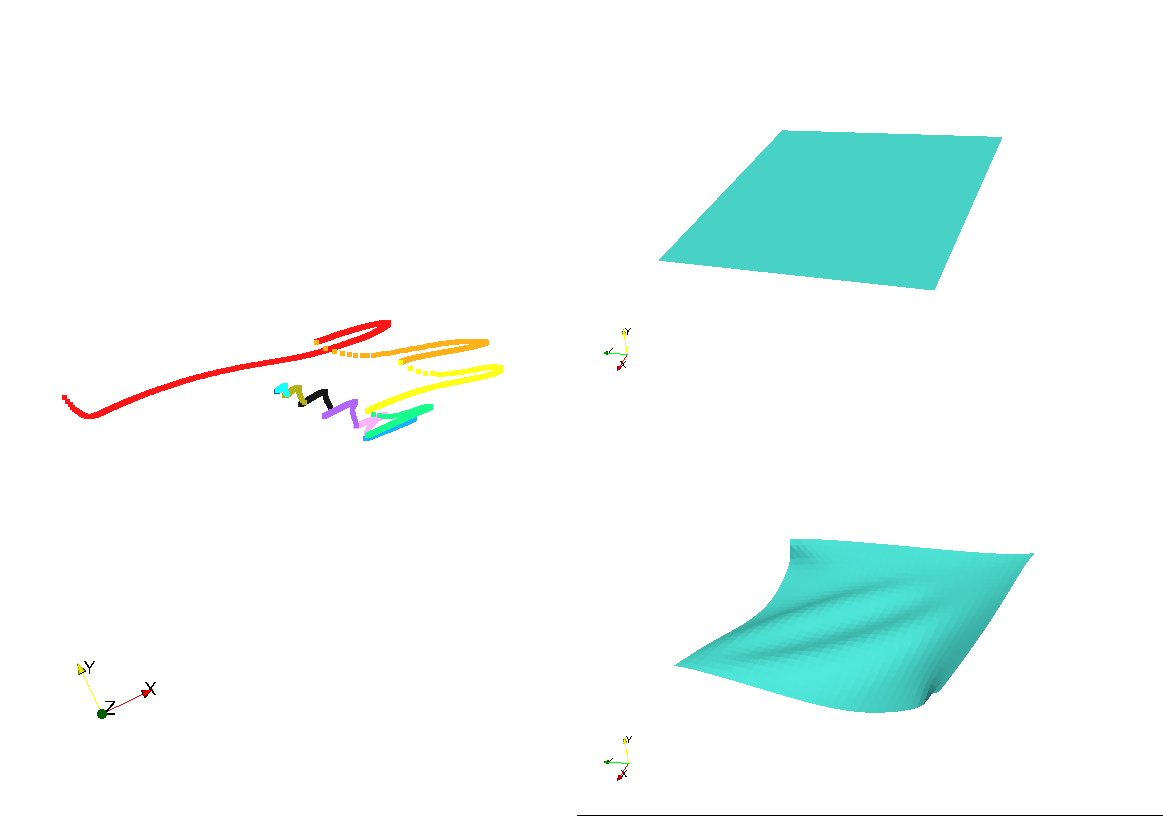
\includegraphics[scale=0.12]{img/mass_spring_rot}};
	\node at (2, -1.3) {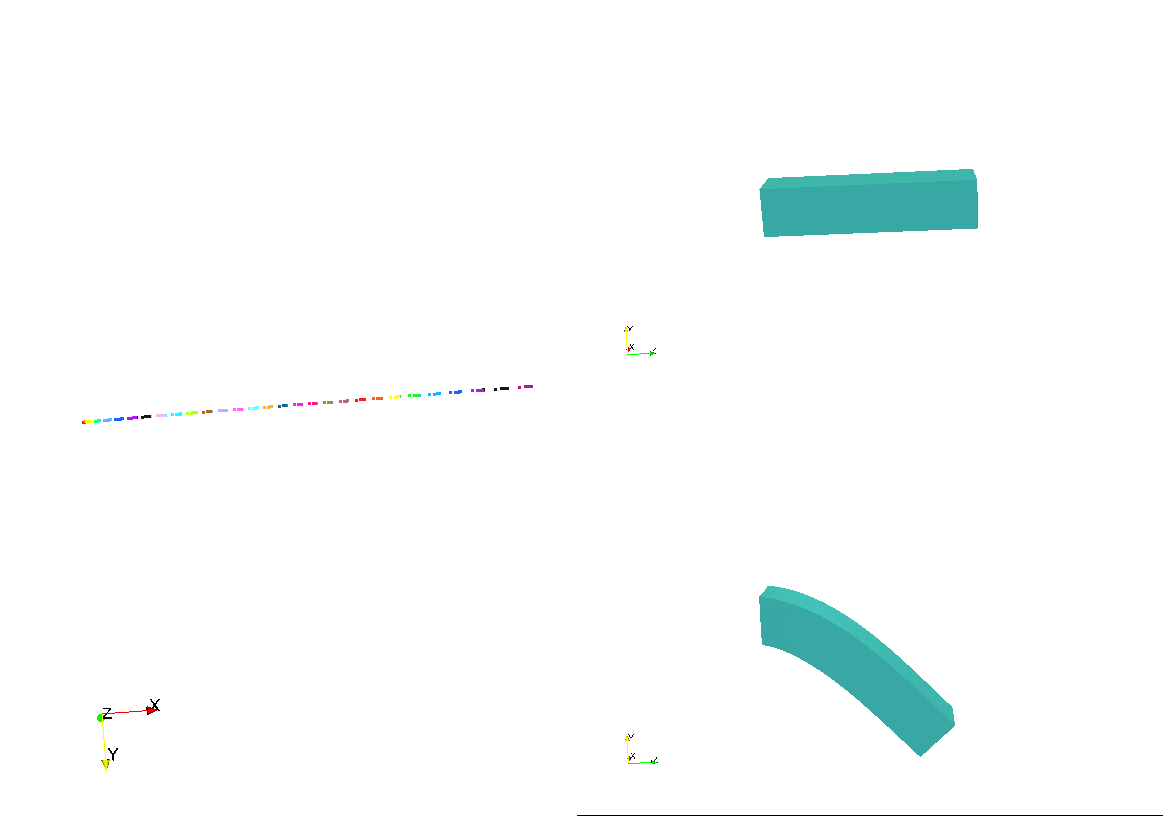
\includegraphics[scale=0.12]{img/tet_rot}};
      }
    }
    \pause
    \pause
    \item Convergence test condition: $\|\nabla E(\BOLD{x})\|_2 \le 10^{-8}$
    \item Do accelerate the convergence by at least one order of magnitude.
    \item Direct+Chebyshev is fastest on CPU.
    \TikzDraw {
      \visible<4> {
	\draw [fill=white, white] (-5, -3) rectangle (5, -0.4);
	\node at (-1.8, -5) {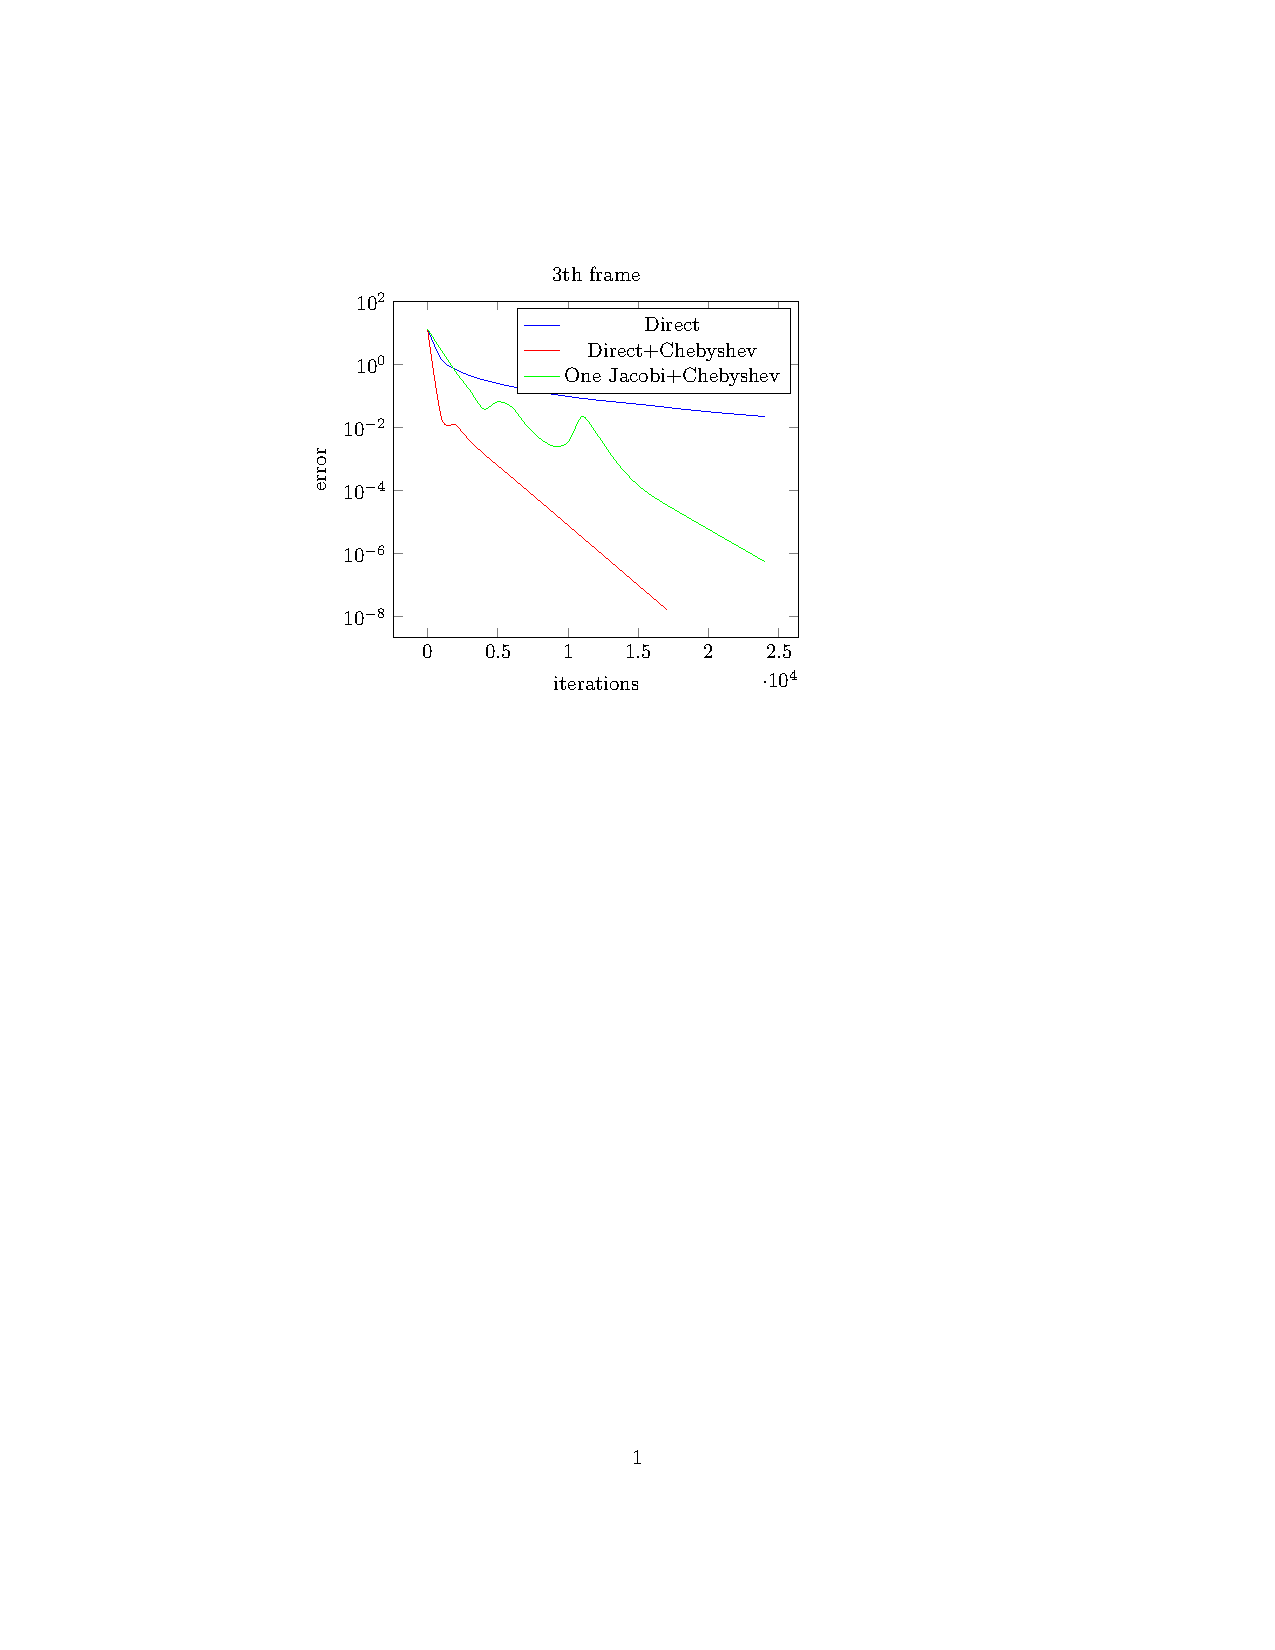
\includegraphics[scale=0.5]{img/plot}};
	\node at (2.5, -5) {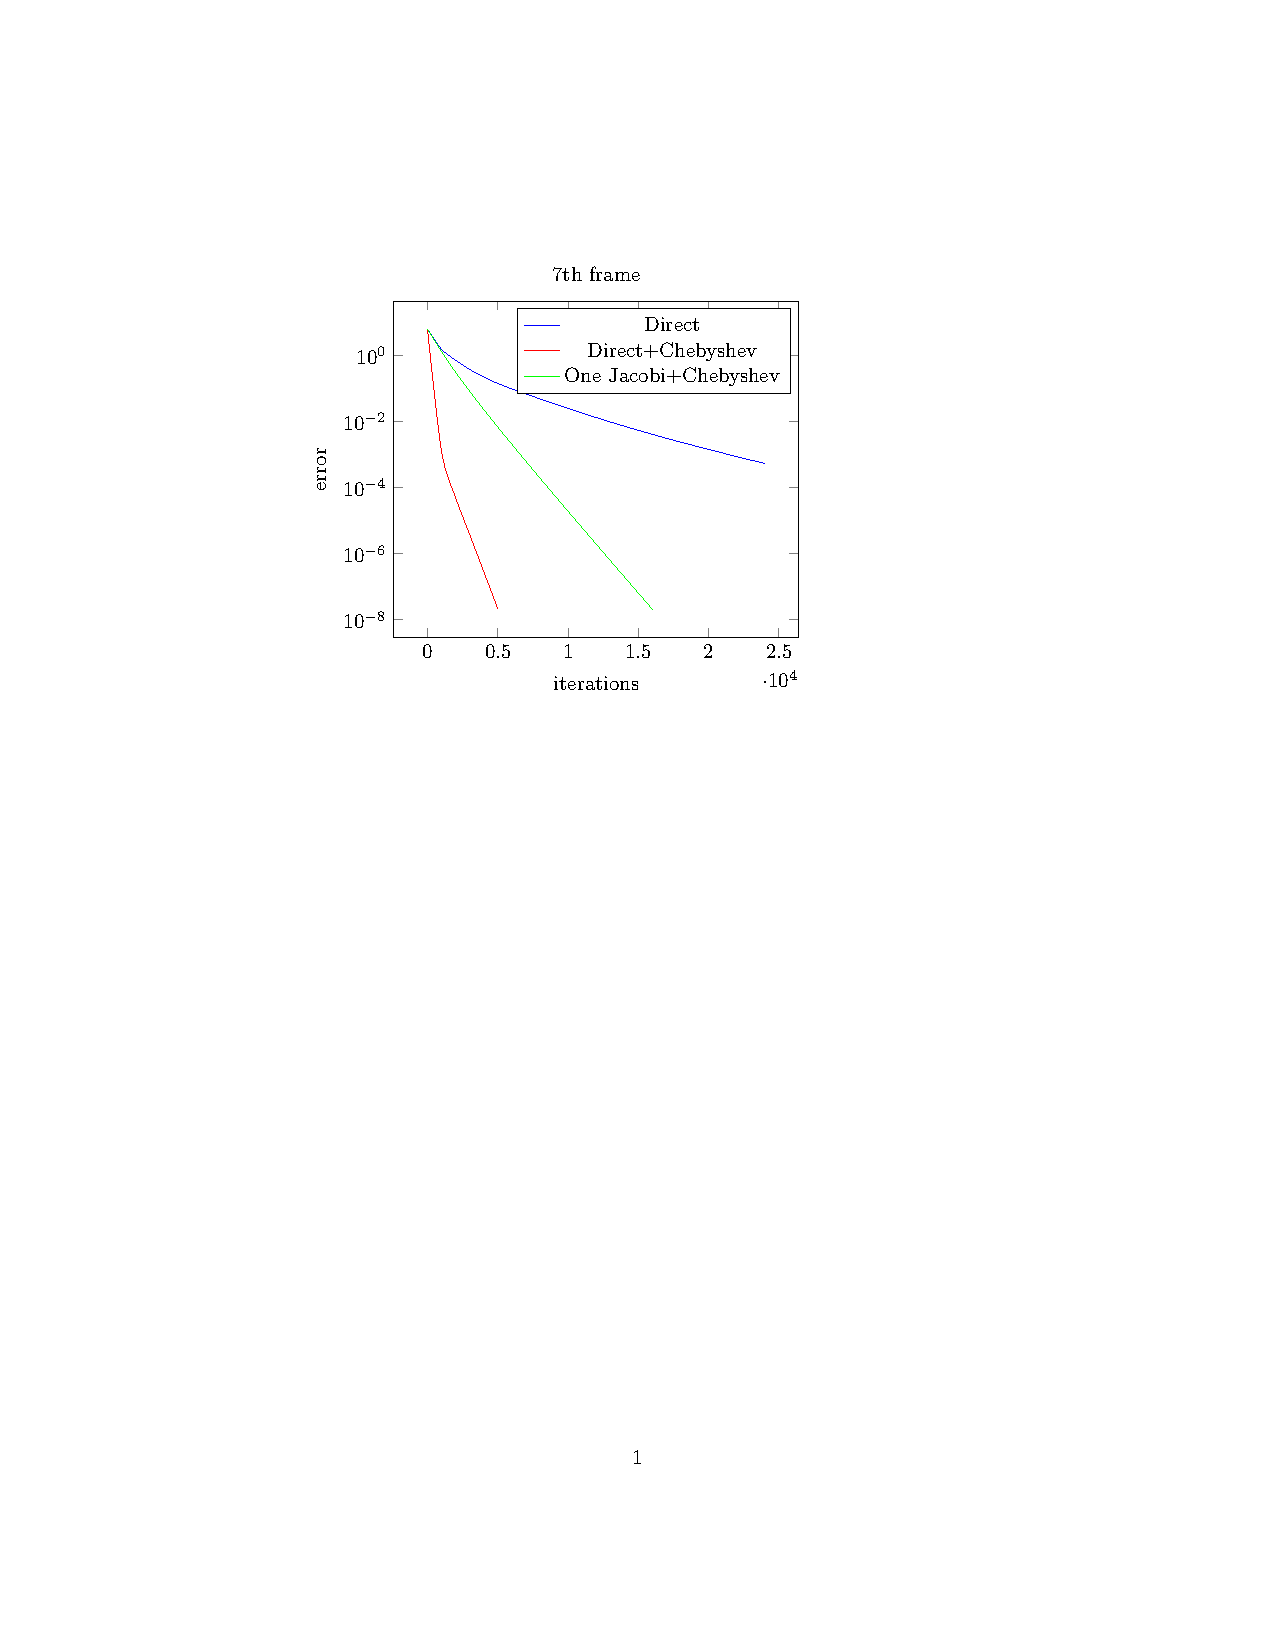
\includegraphics[scale=0.5]{img/plot1}};
      }
    }
    \pause
    \pause
    \item \TODOB{In mass spring, different approaches converged with a little different energy values.} 
  \end{itemize}
  %\gridlines
\end{frame}

\begin{frame}
 \frametitle{Conclusion}
\end{frame}

\begin{frame} 
  \TikzDraw {
    \node at (0, 0.5) {\Huge{Thanks!}};
  }
\end{frame}

\end{document}
